% \chapter{Building Energy Model of Data Centers}
% \label{chp:bem}

\section*{Abstract}	% Section headings need to be upper and lower case.
% -------------------------------------------------------------------------------------------------------------------------------

\addtocounter{section}{1}

\added{Data centers (DCs) have 10 times the power density of conventional buildings. With this density, it is essential that the during the design phase, designers have access to representative building energy models. However, there is a need to have high fidelity building level energy models during the operational phase of DC as-well.

This paper demonstrates a DC building energy simulation that is useful for the operational phase of DCs by implementing network traffic as an indicator of the information technology load. The choice of network traffic profile is superior to the usual hour-day-week schedules an operational model because (1) most data centers serve international users across many time zones. (2) the data center workloads are known to not be stable across time. (3) network traffic is conducive to predicative models based around world events and seasons.}

\deleted{Data centers are the backbone of today\textsc{\char13}s internet based economy. From an energy perspective, in the U.S data centers consume around 2\% of the total energy produced, with 10 times or more power density then conventional office buildings. Through the COVID-19 pandemic, data centers across the globe have seen a disruptive shift in traffic and workload patterns. Given this timely example, it is warranted that data center operators be able to simulate their facilities to verify that their infrastructure can handle these types of shifts in traffic. This research proposes that dynamic computational workloads of data centers can be sufficiently and accurately characterized with current building energy modeling tools to allow such simulations.

The methodology presented in this article couples a network model indicative of internet traffic with the building power load profiles. The effectiveness of such a model is demonstrated by extending the model to five data centers dispersed globally and comparing their results. The framework can be used by architects and designers to assess building energy models of data centers and to provide an indicator of opportunistic thermal headroom during non-design day conditions.}



% -------------------------------------------------------------------------------------------------------------------------------
\section*{Introduction}
% -------------------------------------------------------------------------------------------------------------------------------

\deleted{In 2020 U.S data centers are projected to consume 73 billion kWh \citep{Shehabi16}. This value is significantly curtailed from the trends documented in a 2007 Report to Congress \citep{koomey07}. The report provided evidence of unsustainable energy demands by data centers as the industry expanded, based-on the industry\textsc{\char13}s growth observed from the early 2000’s. Koomey\textsc{\char13}s report was a medium that spread awareness of the problem. Since then various opportunities for energy reduction have been identified and implemented by IT equipment and facility systems architects.

Two specific engineering choices have had profound benefits towards data center energy efficiency. First, proportional power and thermal control of data center components is now enabled across all dimensional scales. An example of a millimeter scale proportional control is of central processing units (CPU) with dynamic frequency voltage scaling (DFVS) \citep{osullivan15}, \citep{barroso18}, \citep{joshi12}.

To appreciate the DFVS’ correlation across the distinct technical domains of computer systems and buildings it should be noted that legacy hardware operations did not proportionally utilize power or cooling with their information technology  (IT) workloads. Most intuitively, this meant that an IT device consumed nearly the same amount of power whether it was idle or being 100\% utilized. The latest generation of IT equipment have much better proportional control enabled by variable fan speeds, variable power draw, and variable heat dissipation resulting from workload dependent power draw enabled with DFVS.  

Second, power and thermal constraints have been relaxed compared to legacy practices. As an example, led by hyper-scale early adopters like Facebook,dual conversion power typologies are now being replaced with bypass systems \citep{Park15}. The removal of dual conversion power systems not only saves capital costs associated with complex uninterruptible power distributions, but it also saves operational expense by requiring power rectification at the IT point of connection only. 

Omission of dual conversion power distribution systems is one example that has been enabled by deep integration across IT and building systems power architectures. Another example is the collaboration between thermal architects of IT and buildings that led to the expansion of the operational environment\textsc{\char13}s thermal psychometric window for IT equipment. An expanded psychrometric window increases the opportunity to exploit free cooling modes across various climate zones \citep{ASHRAETC9.9}. In more aggressive implementations, some data center operators have gone beyond the opportunistic use phase power usage effectiveness optimality and have discarded compressor-based equipment from their cooling plants completely. Compressor-less cooling plants offer significant capital costs savings as-well as the operational energy and maintenance costs \citep{Mulay18}.} 

The power usage effectiveness metric ($PUE$) as defined by Equation~\ref{eq:pue} has been the primary focus for data center facilities architects. 

\begin{equation}\label{eq:pue}
  PUE  = \frac{Total\; Power\; Used\; at\; Facility}{Power\; Consumed\; by\; IT\; Equipment}
\end{equation}

In operations, the facilities and IT parameters change simultaneously together in a continuous sequence, lending to accurate real time evaluations of the $PUE$. However, the continuous states of IT workloads and ambient environmental conditions makes design time PUE calculations complicated. The complications drive data center building designers to quantify PUE at discrete step-wise workload values \added{ (hour-day-week)}. 

Like the PUE calculations, data center building energy models are also reasoned about through these coarse step loads. \added{In the design phase t}\deleted{T}he step-wise inputs are sufficient for two things. First, for sizing equipment which must support the nominal data center capacity in any possible operational condition. Second for producing energy models which are suitable for prescriptive compliance reviews; allowing  municipalities to normalize across different data centers in their jurisdiction. 

However, without accounting for continuous workload profiles these coarse models misrepresent the part-load operations of the data center and inaccurately quantify total energy demands over a time period. The misrepresentation has significant impacts throughout the life of the hardware deployed in these data center facilities. For example without realistic coincident alignment of workloads and ambient conditions, the thermo-electric equipment whose energy use is dependent on workloads and ambient temperatures may be over-sized for significant portion of their operational times. More explicitly, in conditions where the ambient enthalpy is lower then the design day, the additional capacity of the cooling equipment are stranded. 

The proposed simulation in this research will allow for a more realistic evaluation of data center energy use; in-turn exposing the facility's power and cooling equipment headroom for non-design day conditions. These evaluations can facilitate data center operators to opportunistically oversubscribe the IT loads as an extension to the electrical over-subscription \added{leading to free capacity} schemes presented by Li \citep{Li18}.  

The contribution of this work is an IT load aware building energy model that integrates a dynamic time-series of IT power with EnergyPlus. This method can further be expanded by exploiting the real-time headroom at coincident IT load and environmental conditions vs. the design-day capacities of the facilities equipment for opportunistically increasing the supportable IT workloads that are constrained by \deleted{power, leading to free capacity} \added{utility power reservations and back-up power reservations. More explicitly, during the part load operations of the cooling plant when their electrical demand is lower then their design values, the headroom in power from the cooling equipment can be safely supplied to IT equipment. The rerouting of the available power increases the supportable IT load and essentially 'free capacity' beyond the design values of the IT load}.

As an example of free capacity, consider a design day dry-bulb temperature of \deleted{110$^{\circ}$F}\added{105$^{\circ}$F}. When a peak in IT workload occurs on a more favorable day, say 95$^{\circ}$F, the computer room air conditioner heat rejection equipment needs less than 50\% of the designed power value \citep{liebert20}. With a slight modification in the electrical infrastructure, this difference can opportunistically be allocated to IT workloads. However slight the the electrical modification, the decision is most cost effectively made during the design phase of the the facility.

\deleted{This article first provides a background for the need of IT coupled data center building energy models and discusses similar works. Then a novel simulation methodology is proposed for extending the existing data center modeling capabilities of EnergyPlus to allow for dynamic IT workload profiles in it. Using the proposed method, two simulations are performed and their comparisons are discussed. The first of the two models serves as a baseline, where the peak IT load is constant throughout the year. In the second simulation, a dynamic IT workload is expressed. A comparison of the results are then presented in the Results from Proposed Method section. The article concludes with a summary of the work and outlines future research that leans on this model.}

% -------------------------------------------------------------------------------------------------------------------------------
\deleted{\section*{Background}}
% -------------------------------------------------------------------------------------------------------------------------------

\deleted{Over the last 15 years, the deployment paradigm of data centers has transformed from monolithic deployments of high-end devices to heterogeneous deployments of cost-efficient commodity equipment that dwarf the their predecessor in all dimensional scales. With an appropriate title, in Warehouse Scale Computer Barroso et al. describe their data center design and operational experiences in this new paradigm \citep{barroso18}. The work provides details from the software platforms to the industrial sized power and cooling plants found at mega-Watt scale data center campuses. This work provides compelling financial incentives for designs and operations that prioritize proportional energy use at these massive scales. Furthermore, Barroso provides explicit workload profiles from real data centers that lend themselves to opportunistically oversubscribe the capacity of the mechanical and electrical infrastructure in proportion to the IT workloads.

It is evident by the preceding discussions that energy efficiency of data centers is dependent on the proportional power management across all components found in them. However, the PUE metric presented above does not capture the end to end electro-mechanical efficiency of data centers as it misses the IT inefficiencies. For IT devices, several methods for enhancing the proportional power management have been summarized by O\textsc{\char13}Sullivan \citep{osullivan15}. O\textsc{\char13}Sullivan presents design solutions for those methods and demonstrates that through workload proportional computing, it is technically feasible to optimize the end to end electro-mechanical efficiency of the hardware. The control feedback loops that O\textsc{\char13}Sullivan describes also lend themselves to be leveraged by building systems. As an example, return air temperature readings at air handlers can be supplemented with input power demand values to more effectively control air handling fan speeds and their cooling stages. 

Awareness of the total power demands jointly by the building system\textsc{\char13}s and the IT telemetry leads to another area of integration, power capping. Power capping throttles the CPU power cycles, similar to load shedding schemes implemented by power utility companies for consumer energy use. A novel power capping strategy is proposed by Li \citep{Li18}. Li\textsc{\char13}s power capping methods provide a means for building systems to actively exploit the device level power management capabilities of Intel’s CPU Node Manager feature (\citep{intel15}. Intel\textsc{\char13}s CPU Node Manager enables the data center infrastructure telemetry to observe building telemetry (ie from power meters on rack power strips) and throttle the CPU when the workloads demands encroach the facilities power, risking an upstream circuit-breaker trip.

Given the various operational interdependence between building and IT systems, traditional building energy modeling techniques have failed to suffice for data centers \citep{Beatty15}. Beatty\textsc{\char13}s critique resonates with the three influential data center energy evaluation methods. Those methods either are directly enforced or adopted through reference by authorities having jurisdiction across the US. 

The first and most influential method is ASHRAE 90.4, the Energy Standard for Data Centers (ASHRAE, 2019). Compliance with the standard can be achieved through prescriptive or performance-based methods. EnergyPlus simulations are one of the approved methods for performance-based compliance along with spreadsheet-based methods. Regardless of the method, the standard allows various subsystems to be isolated for compliance based on whether they are mechanical or electrical load components (MLC/ELC) which fall back on prescriptively defined threshold values.

The second influential method is a part of the certification process for the US Green Building Council\textsc{\char13}s LEED program. LEED requires prescriptively defined performance calculations to validate compliance \citep{LEED16}. Compliance with the LEED method is done through a spreadsheet tool, where designers input their data center IT characteristics along with the properties of the IT power distribution system. The strict prescriptive boundary set by LEED accounts for the electro-mechanical efficiency at discrete design points of specific devices but does not account for the computational workloads. The computational workloads are known to significantly influence IT equipment power draw \citep{marculescu20}.  

The third method, adopted by many power utility companies for compliance with their rebate program comes from the Pacific Gas and Electric Company (PGE). PGE method mandates an documented IT load profile to indicate the part load conditions, where the profile is established with 1-month of trend data for new construction. In industrial practice however, it takes several years to fully populate a data center with equipment and data center workloads, like the weather, have seasonal periods of cyclic behavior \citep{zhuang15}.}

% -------------------------------------------------------------------------------------------------------------------------------
\section*{Similar Works}
% -------------------------------------------------------------------------------------------------------------------------------

As described above, PUE is not a full proof metric for data center energy efficiency. By acknowledging that PUE does not account for IT equipment efficiency, Perolini provides a coordinated control strategy across IT workload and building infrastructure based on network queuing theory \citep{parolini12}. Perolini logically composes a set of IT systems and supporting infrastructure as a singular cyber-physical system network graph. Hierarchically structured quality of service (QoS) values is common among Perolini and Li \citep{Li18}. Both dynamically tune IT with the facilities infrastructure systems. The fundamental difference between these two works is that Li considers the IT workload as the controlled variable bound by the facility\textsc{\char13}s systems and Perolini considers the cooling equipment as the controlled variable bound by the IT workload. In their recognition of some data center workloads as being preemption tolerant and others as time sensitive, these methods allow over-subscription of both power and thermal capacities without any service level performance degradation. 

Data center cooling systems have been algorithmically coupled with data center IT workloads by Wei in \citep{wei17}. They use a reinforcement learning agent that is aware of the data center\textsc{\char13}s thermal state in real-time. The agent acts as a controller of the HVAC equipment and respective IT traffic balancer, where the balancer migrates work between two or more data centers. In the work they demonstrated that when given a state-action pair and an objective function; the agent takes a control action in a given state to reduce power while allowing the IT system to meet it\textsc{\char13}s performance objective in terms of processing latency. The state-action pairs are optimized with an objective function that values the power demand along with a IT performance metric at a given time-step. Wei\textsc{\char13}s work was limited to data centers located in mixed use building,where the cooling system had some fungibility with other parts of the building, which allowed waste energy from the data center to be reclaimed to heat the other parts. Nonetheless, their work is similar to this research in that it also integrated EnergyPlus together with Python.

% -------------------------------------------------------------------------------------------------------------------------------
\section*{Methodology}
% -------------------------------------------------------------------------------------------------------------------------------

In this section a dynamic workload-profile based energy simulator is introduced and a simulation is described in detail. The simulator allows Python algorithms to interact with EnergyPlus through the Building Controls Virtual Test Bed (BCVTB) \citep{wetter16}. The BCVTB interface from Gym-EPlus \citep{zhang19} is used to implement the interaction. Functionally, the Python agent handles programmatic logic about the IT workloads. Python is chosen for the interface function due to its flexibility and the the granular level of program control and EnergyPlus is chosen due to it\textsc{\char13}s established efficacy with building modeling.

EnergyPlus is the US Department of Energy\textsc{\char13}s state-of-the-art building modeling software. It features an extensible physics-based building thermodynamic and psychrometric modeling engine to simulate sub-hourly energy demands and occupant comfort values. Data-centers have been explicitly supported in EnergyPlus since release of Version 8.3.0. As shown in Figure 1, the proposed simulator uses Python as an external interface to reset the Data center load for each time-step. In the subsequent modeling time-step, the EnergyPlus models runs with the externally revised variables.The basic process loop of the simulator is illustrated in Figure~\ref{fig:dyna-bem}. 

\begin{figure}
\centering
\includegraphics[scale=.10]{img/agent_bem.png}
\caption{Dynamic Process Flow between EnergyPlus and the Python Agent.}
\label{fig:dyna-bem}
\end{figure}

The data center building is configured in EnergyPlus with an IT load density of $2\frac{kW}{m^2}$. The remainder of the model is based on Moriyama\textsc{\char13}s data center model from \citep{moriyama18}. Moriyama uses a full suite of mechanical cooling equipment and configures them with the SequentialLoad setting. By using SequentialLoad in the EnergyPlus IDF, each piece of equipment ramps up in the order listed. 

Without the Python feedback loop, EnergyPlus is a hermetic suite in which simulation run-parameters are defined in a configuration file; namely the IDF. In the default case, EnergyPlus modeling workflow serially runs the simulations \deleted{and then users get to review the results of each simulation at} \added{to} completion. Iterating on the parametric values requires \added{manual} editing of the IDF file and re-running of the entire simulation. This proposed simulation specifically defines a loop in Python which iterates over a list of load coefficients derived from the network traffic corresponding to the cooling load for each simulation time step.   

The traffic profile of an internet service is an intrinsic property of the service. Characterizing the traffic profiles requires granular data that spans across a wide temporal range. However, due to the competitive nature of the internet industry such data that allows for building level traffic profiles is not publicly available. Therefore, in this research a network traffic simulator is created. The objective for the simulator was to represent a globally distributed online platform indicative of real world user demand. To represent a global service, the load factors in this article reflect visits to 145,063 Wikipedia pages over an 18-month period as provided by Kaggle \citep{kaggle17}.

One issue with the Kaggle data set is that it just provides a time series of page visits that is agnostic of source location (ie user location) or serving data center. For evaluating data center level workloads, the pages were mapped to a data center as part of a pre-processing step of this research. The pre-processing required parsing the raw URL strings and parsing out it\textsc{\char13}s language hash markers. Then, countries where these languages are the official languages were mapped to the nearest Wikipedia data center to indicate the traffic to each data center.  This resulted in the seven languages being routed by a minimum distance function from any country that they are the official language to the nearest data center site. Treating each of the seven languages as a service allows this research to have an abstraction of the (Moriyama , et al., 2018)service which is intuitive to reason about as indicated in Figure~\ref{fig:lang2dc}. 

To validate the impacts of resetting the proportional load factors, two specific simulations were run for each of the data centers from Figure~\ref{fig:lang2dc} The first is the novel dynamic load simulation and second configured as in \citep{moriyama18}. In both simulations nominal power density of the data center is set to 2kW/m2 and the auto-sizing feature is enabled for all HVAC equipment. 

\begin{figure}.
\centering
\includegraphics[scale=0.45]{img/lang2dc_curve.jpg}
\caption{Sum of English, French, German, Mandarin, Spanish, Russian, and Japanese traffic to each of the 5 data center locations.}
\label{fig:lang2dc}
\end{figure}

In the proportional load simulation, the traffic load factor is pulled in by the Python program and at each time step it is passed to EnergyPlus. The load factor that is passed represents the CPU loading of servers, where CPU loading is a dominate energy consumer of IT equipment but it’s not the only power consumer. In EnergyPlus IT equipment always consumes a near constant rate of energy for hard disks, random access memory, fans and other parts regardless of the load. This constant rate is approximately 30\% of the power density, in line with industry practices \citep{barroso18}. 

\textit{Algorithm} \ref{Service Profile} indicates how the the service demand profile is generated. It is based on Kaggle's web-traffic data-set $(K)$ which is a time-series of the count of visits $(v)$ to 145,063 Wikipedia pages distributed across seven languages $(l)$ at daily intervals \citep{kaggle17}. In this work  pages $(p)$ are aggregated together by language and classified as a common service. $P_l$ is a list of all pages with the language $l$. The subscript $d$ represents individual data centers.  The demand for the service at a particular data center is obtained by the average quantile visits to the pages of the respective language as indicated by $P_{l}[d]$.  Figure~\ref{fig:lang2dc} illustrates the service profile for the data range and notes the seven languages. The y-axis is the number of page views on a $1e^8$ scale, the x-axis spans the date range, and the curves represent each of the seven languages.

\begin{algorithm}
\caption{Service Profile}
\begin{algorithmic}[1]
\REQUIRE{$K$} %Time series
	\FOR{$p$ in $K$} % Each Page in the time T
		 %For each lanugauge in T
		\STATE{$P_l = empty[$ $]$} % Create a unique table for each lanuage
		\STATE {$P_{l}[l] \gets p_l == l$  } % Populate matching langauge intot he luange table
		\FOR{$d$ in $range(K_d)$}
			\STATE {$P_{l}[d][quantile(v)] \gets \sum{P_{l}[l][d]}$} %Sum the visits, v per day to get service profile
	\ENDFOR
	\ENDFOR
\end{algorithmic}
\label{Service Profile}
\end{algorithm}

Next we discuss the results from the simulations. 

% -------------------------------------------------------------------------------------------------------------------------------
\section*{Results}
% -------------------------------------------------------------------------------------------------------------------------------

Two simulations for each of the five data center locations from Figure~\ref{fig:lang2dc} were run. The total annualized energy use of the two models is plotted for comparison in Figure~\ref{fig:total_energy_comp}. The purple bars indicate the simulations in which the CPU loads are reset at each time-step (RL), and the green bars indicate simulations without interactive resetting of the loads (NoRL). For Singapore (sin), San Francisco (sfo), and Ashburn (ash) the RL simulations result in higher annualized energy compared to the NoRL model. While for Amsterdam (ams) and Carrolton, TX (car), the RL model results in lower energy demand compared to the statically configured load from the NoRL simulation.

\begin{figure}.
  \centering
  \includegraphics[scale=0.45]{img/total_energy_comp.png}
  \caption{Total Site Energy Difference between statically configured IT load and dynamically reset IT loads.}
  \label{fig:total_energy_comp}
  \end{figure}

The variations in the relative energy demands between the two models can be attributed to the CPU load profiles as illustrated in Figure~\ref{fig:cpu_comps}. The figure illustrates time series plot of each of the five data centers analyzed through the RL simulations. The x-axis indicates the hour of the year and the y-axis indicates the CPU load for each respective data center. Examining the profiles for each data center they all appear quite distinct from a one another. Carrolton and Ashburn appear to have strong seasonal patterns. Amsterdam and Singapore data centers show irregular oscillations in demand throughout the year. The San Francisco data center has a constant line. This constant demand is due to the load not varying much from the peak capacity in the traffic profile that was used for the site. 

In contrast to the distinct CPU load profiles of the RL loads as discussed above, with static schedule configuration of IT load profiles used in the NoRL models, the CPU loads at all the data centers are identical to each other. This configuration of the NoRL models is based on default data center load schedule as used by \citep{moriyama18}. The static property of the NoRL model is also indicated in \ref{fig:cpu_comps} by the gray band. The gray band is actually composed of line curves that oscillate diurnally.


\begin{figure}
  \centering
  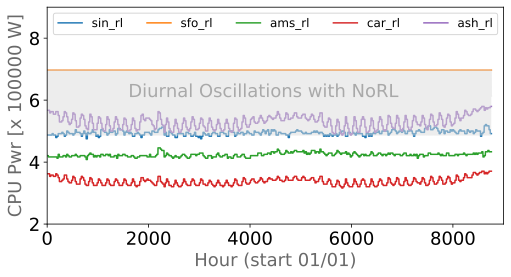
\includegraphics[scale=0.45]{img/cpu_comps.png}
  \caption{Time series of the total CPU power at each data center (see legend). Gray area indicates the daily demand cycle that the IT equipment creates with NoRL.}
  \label{fig:cpu_comps}
  \end{figure}

  Given this understanding of the cyclic loads, the relative variance between the RL and NoRL simulation’s total energy results can be reasoned about by considering the profile of San Francisco data center as an extreme example. San Francisco’s RL model does not vary the CPU load, whereas the NoRL model does. With the constant peak load, the San Francisco data center’s RL simulation indicates higher utilization than the NoRL model therefore demanding more power.


%-------------------------------------------------------------------------------------------------------------------------------
\section{Discussion}
% -------------------------------------------------------------------------------------------------------------------------------
To reason about the EnergyPlus RL results from Figure~\ref{fig:total_energy_comp} for total energy, the San Francisco site again serves as an example. In the figure, the total site energy used for the annual model is $1.19 \times 10^7$kWh. Through the course of 8,760 hours the power demand for the data center is 1,359 kWh on average; translating to an annualized PUE value of approximately 1.36 due to the base IT load density of $2 kW/m^2$ (with a network load coefficient set to 1 for all hours). The PUE values of the other sites are more complex to reason about without further processing of the data, as they all operate at part load conditions.

In this research the network traffic serves as a proxy for CPU utilization. In practice the network traffic and CPU have complex correlations that can\textsc{\char13}t be generalized with the presented approach. In production data center environments representative correlations can be obtained between network traffic, the IT workloads the the traffic instantiate, and the workload\textsc{\char13}s CPU demand. However, proving such correlations is out of scope of research.

This research assumes that all the facilities are of the same size in terms of power. From looking at Figure~\ref{fig:lang2dc}, San Francisco site has a much lower traffic profile than Haarlem. To claim that the same power capacity handles this range of traffic another assumption is made. This assumption is that the CPU-Network ratio varies from site to site. For example a bit (digital bit) of network traffic generates 40 times as much CPU workload in San Francisco as it does in Haarlem. This is a realistic condition in data center fleets were have different generations of IT hardware in operations at various data centers. Or this condition can be encountered when software optimizations to specific workloads are done for targeted consumer markets that are geographical segregated. Nonetheless, since the network coefficient is bound between 0 and 1, and network-workload-CPU model can be supported in the same framework. 

\added{The discussion on opportunistically using 50\% of the provisioned power from the cooling equipment to power the IT equipment requires some clarifications. First, the 50\% claim is based on nameplate full load amps (FLA) for two different dry-coolers that are matched with a 105kW indoor computer room air conditioner. One of the dry-coolers is rated at 95$^{\circ}$F and the other is rated at 105$^{\circ}$F \citep{liebert20}. The FLA for these units are 14 Amps and 28 Amps respectively. Physically this translates to breaker sizes, wires sizes, utility power feed reservations, and back-up generator reservations decisions being made using this value.  Second, with the claim it is assumed that the power draw scales similarly cross both units.

This is a naive assumption and such a practice is not suitable for the design phase building energy models where equipment must be sized for worst case conditions. However, the claim suffices to demonstrate that on non design days there is stranded power in terms of the physical capabilities of the electrical infrastructure. For a building class where its utility is measured by IT power density; any opportunistic usage of power is highly valuable. As a concrete example, when the part load of the dry cooler is known for future states in time, major capacity constraints in DC such as the utility power reservations and back up generator reservations can be relaxed during that time range. This would allow the IT to be oversubscribed relative to its design conditions, yet the building would still be within its overall power envelope. 
}

% -------------------------------------------------------------------------------------------------------------------------------
\section*{Conclusion}
% -------------------------------------------------------------------------------------------------------------------------------
There are two notable benefits of resetting the IT load values outside of the IDF file. First, defining load values for each hour in the IDF file is toilsome and error prone. The toil of entering values for each simulation time-step would require 8,760 entries in the file. This increases the chance of introducing errors into the simulation. Second, the external definition allows more sophisticated logic to control the time-step variables. In this article, only the IT load factors were reset, none-the-less the same interface can reset many other simulation run-parameters with similar logic. An example of a feedback logic is reinforcement learning, which can be framed to globally optimize the systems and is an topic for future research. 

The traffic profile used in this article are representative of a globally distributed service’s user facing workloads and suffices for purposes of demonstrating the dynamics of data center operational loads. Each real-world service will have a unique profile resulting from a combination of critical and opportunistic back-end workloads. The modular construction of this model is conducive for incorporating the other workloads and being inclusive of back-end workloads.